\documentclass[11pt]{article}

% Pacotes extras necessários
\usepackage{amsmath}
\usepackage[lmargin=0.7in, rmargin=0.7in, tmargin=0.5in, bmargin=0.5in, includehead, includefoot]{geometry}
\usepackage{amsfonts}
\usepackage[utf8]{inputenc}
\usepackage[portuguese]{babel}
\usepackage{graphicx}
\usepackage{fancyhdr}
\usepackage{setspace}

\graphicspath{ {./images/} }

% Sets para outras partes
\setlength{\parindent}{0pt}
\setstretch{1.25}
\DeclareMathOperator{\sen}{sen}

%% Facilidades
%% -- Laplace
\newcommand{\Lap}[1]{\mathcal{L}\left\{#1\right\}}

%% -- Fourier
\newcommand{\Fou}[1]{\mathcal{F}\left\{#1\right\}}

% ------- Estilo do trabalho -------- %
\fancypagestyle{capa}{
    \fancyhf{}
    \renewcommand\headrulewidth{0pt}
    \fancyfoot[C]{
        Rio de Janeiro\\
        2022
    }
}

\pagestyle{fancy}
\fancyhead{}
\fancyhead[L]{\thepage}
\fancyfoot{}
% ----------------------------------- %

% Dados do Grupo
\title{Sinais e Sistemas - Trabalho 4 - Avaliação 8}
\author{
    \textbf{Grupo 2}\\
    Leonardo Soares da Costa Tanaka\\
    Matheus Henrique Sant Anna Cardoso\\
    Theo Rudra Macedo e Silva
}
\date{}

\begin{document}
\maketitle
\thispagestyle{capa}
\newpage

\textbf{1.) Abaixo, use o número do grupo como o valor do parâmetro $p$. Entre no Octave com \texttt{B = [0 ; 0 ; 1], C = [1 0 0], A = [0 1 0 ; 0 0 1 ; (-2p) (-2p + 2) (-p + 2)]}, e serão criadas as matrizes $A, B \text{ e } C$ de uma equação dinâmica. Com auxílio do \texttt{help}, pesquise e use os comandos \texttt{eig} para calcular os autovalores e \texttt{ss} para criar um sistema de espaço de estados.}

Matrizes relativas ao \textbf{Grupo 2 (p = 2)}:

\texttt{B = [0 ; 0 ; 1], C = [1 0 0], A = [0 1 0 ; 0 0 1 ; -4 -2 0]}

\textbf{(a) Encontre o polinômio característico $\Delta(s)$ associado;}

\[
\Delta(s) = det(sI - A) = det\left(
\left[ {\begin{array}{ccc}
  s & 0 & 0 \\
  0 & s & 0 \\
  0 & 0 & s \\
\end{array} } \right]
-
\left[ {\begin{array}{ccc}
    0 & 1 & 0 \\
    0 & 0 & 1 \\
    -4 & -2 & 0 \\
  \end{array} } \right]
  \right)
  =
  \left| \begin{array}{rcr}
    s & -1  & 0 \\ 
    0 & s & -1 \\
    4 & 2  & s \\
  \end{array}
  \right|
  = s^3 + 2s + 4
\]

\textbf{(b) encontre a função de transferência $T(s)$ associada, manualmente e pelo Octave (descubra como);}
\[
  T(s) = C(sI - A)^{-1}B =
  \left[ {\begin{array}{ccc}
    1 & 0 & 0 \\
  \end{array} } \right]
  \left[ \begin{array}{rcr}
    s & -1  & 0 \\ 
    0 & s & -1 \\
    4 & 2  & s \\
  \end{array} \right]^{-1}
  \left[ {\begin{array}{c}
    0 \\
    0 \\
    1 \\
  \end{array} } \right]
  \\
=
\] 
 
\[=
  \left[ {\begin{array}{ccc}
    1 & 0 & 0 \\
  \end{array} } \right]
  \left[ \begin{array}{rcr}
    -\frac{s^2 + 2}{-s^3-2s-4} & -\frac{s}{-s^3-2s-4}  & -\frac{1}{-s^3-2s-4} \\ 
    \frac{4}{-s^3-2s-4} & -\frac{s^2}{-s^3-2s-4} & -\frac{s}{-s^3-2s-4} \\
    \frac{4s}{-s^3-2s-4} & \frac{2s+4}{-s^3-2s-4}  & -\frac{s^2}{-s^3-2s-4} \\
  \end{array} \right]
  \left[ {\begin{array}{c}
    0 \\
    0 \\
    1 \\
  \end{array} } \right]
  =
  \] 
  \[
    =
  \left[ {\begin{array}{ccc}
    -\frac{s^2 + 2}{-s^3-2s-4} & -\frac{s}{-s^3-2s-4} & -\frac{1}{-s^3-2s-4} \\
  \end{array} } \right]
  \left[ {\begin{array}{c}
    0 \\
    0 \\
    1 \\
  \end{array} } \right]
  = \frac{1}{s^3 + 2s + 4}
\]

Bastou, agora, encontrarmos a função de transferência utilizando a ferramenta Octave. Para tal, foi feito o programa a seguir:
\begin{verbatim}
%% Dados Iniciais
A = [0 1 0 ; 0 0 1 ; -4 -2 0];
B = [0 ; 0 ; 1];
C = [1 0 0];
%% Carregando o pacote de controle
pkg load control;
%% Sistema de espaço de estados
sys = ss(A, B, C);
%% Função de transferência
SYS = tf(sys)
\end{verbatim}

Tendo por saída, a mensagem com a função de transferência:
\begin{verbatim}

                  1
y1:  ----------------------------
     s^3 + 2.22e-16 s^2 + 2 s + 4
\end{verbatim}
Perceba que existe um coeficiente maior que zero para o termo ao quadrado. Porém, este é desprezível.

Ficamos, pelo Octave, com a função de transferência dada por:
\[y_1 = \frac{1}{s^3 + 2.22 \times 10^{-16} s^2 + 2s + 4} \approx \frac{1}{s^3 + 2s + 4}\]

\textbf{(c) encontre a resposta ao degrau (comando \texttt{step}) para $y \text{ e } x$;}

Aqui, precisamos utilizar, novamente, o Octave.

\begin{figure}[h]
  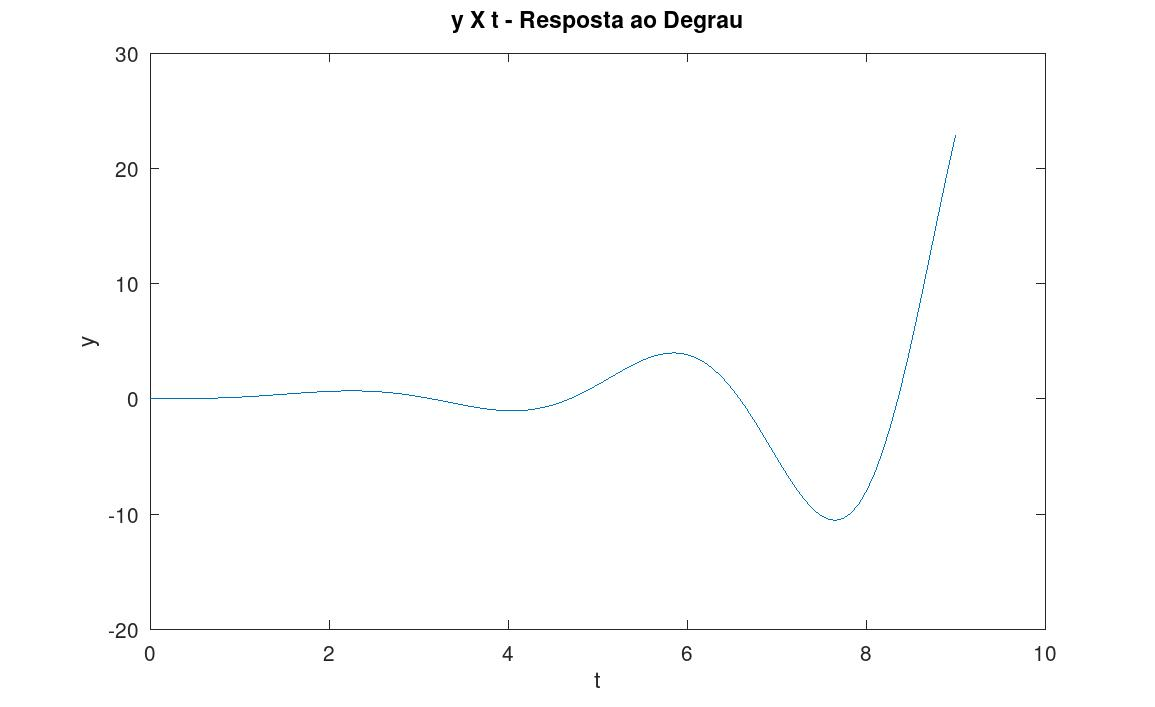
\includegraphics[scale=0.3]{plot1c1.jpg}
  \centering
\end{figure}
\begin{figure}[h]
  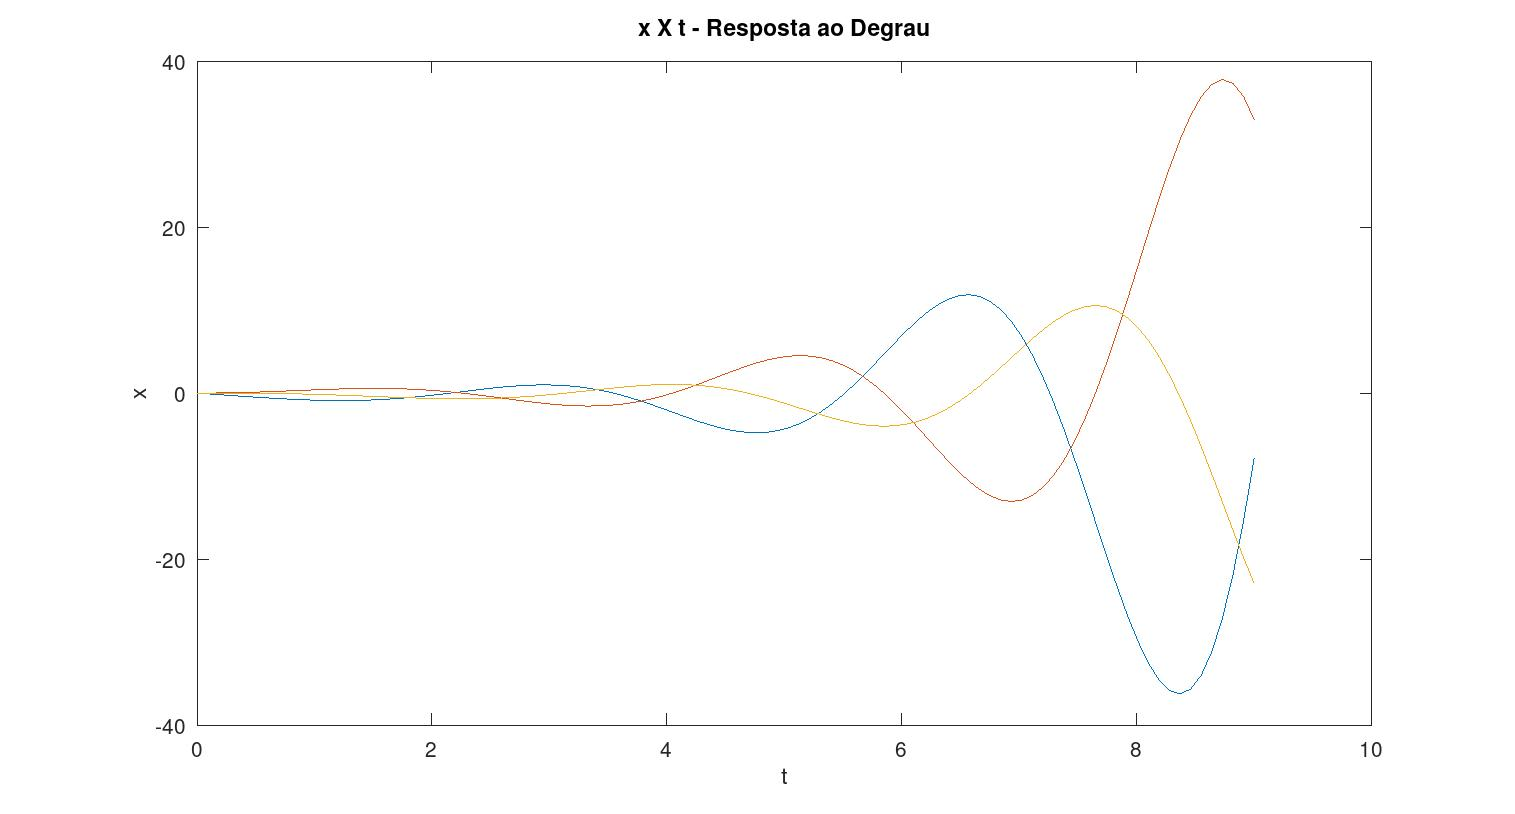
\includegraphics[scale=0.25]{plot1c2.jpg}
  \centering
\end{figure}

\textbf{(d) encontre manualmente os autovetores;}

Vamos encontrar as raízes de $\Delta(s)$ que são os autovalores de $A$. Para isso, podemos utilizar a função \texttt{eig} no Octave para encontrá-los. Dessa forma, encontramos os seguintes valores:
\begin{align*}
  \lambda_1 &= -1.1795;\\
  \lambda_2 &= 0.5898 + j1.7445;\\
  \lambda_3 &= 0.5898 - j1.7445
\end{align*}

Chamando de $\lambda$ quaisquer uma das três raízes, teremos que:
\begin{align*}
  \begin{bmatrix}
    0 & 1 & 0\\
    0 & 0 & 1\\
    -4 & -2 & 0
  \end{bmatrix}
  \begin{bmatrix}
    \alpha\\
    \beta\\
    \gamma
  \end{bmatrix}
  =
  \lambda
  \begin{bmatrix}
    \alpha\\
    \beta\\
    \gamma
  \end{bmatrix}
\end{align*}

ou
\begin{align*}
  \begin{cases}
    \beta  &= \lambda \alpha\\
    \gamma &= \lambda \beta\\
    -4\alpha - 2\beta &= \lambda \gamma
  \end{cases}
  &
  &
  \begin{cases}
    \alpha &= \alpha\\
    \beta  &= \lambda \alpha\\
    \gamma &= \lambda^2 \alpha
  \end{cases}
\end{align*}

Ficamos, com um padrão para os autovetores:
\begin{align*}
  \alpha
  \begin{bmatrix}
    1\\
    \lambda\\
    \lambda^2
  \end{bmatrix}
\end{align*}

Temos, finalmente, como autovetores, os seguintes vetores:
\begin{align*}
  v_1 &=
  \begin{bmatrix}
    1\\
    -1.1795\\
    1.39122
  \end{bmatrix}
  &
  v_2 &=
  \begin{bmatrix}
    1\\
    0.5898 + j 1.7445\\
    -2.6954 + j 2.0578
  \end{bmatrix}
  &
  v_3 &=
  \begin{bmatrix}
    1\\
    0.5898 + j 1.7445\\
    -2.6954 - j 2.0578
  \end{bmatrix}
\end{align*}

\textbf{(e) escreva a REN seguindo o exemplo completo na nova versão dos slides094pwd.pdf a partir do slide 83;}

\textbf{(f) usando o comando \texttt{initial} encontre a REN ($y \text{ e } x$) para $x_0$ colocado em um ponto da matriz $V$;}

\textbf{(g) idem para $x_0$ como uma combinação linear das colunas da matriz $W$.}


%% ------------------------------------------------ %%
\vspace{\baselineskip}

\textbf{2.) Um oscilador ideal com duas massas, molas e sem atritos e/ou amortecimentos é descrito por $\ddot{y_1}(t) + 2\omega_1^2 y_1(t) = \omega_1^2 y_2(t)$ e $\ddot{y_2}(t) + 2\omega_2^2 y_2(t) = \omega_2^2 y_1(t)$. Use a escolha $x_1 = y_1; x_2 = \dot{y_1}; x_3 = y_2; x_4 = \dot{y_2}$ para variáveis de estado, ou qualquer outra, e considere $\omega_1 = \omega_2 = \omega_0$.}

\textbf{G2: } $\omega_0 = 2$.

\textbf{(a) Encontre a matriz de estados $A$, seu polinômio característico $\Delta(s)$;}

\textbf{(b) os autovalores (faça $\lambda_1; \lambda_2; \lambda_3; \lambda_4;$ pares complexos conjugados) e, manualmente, os autovetores $v_1, v_2, v_3, v_4$;}

\textbf{(c) escreva a expressão da REN: $x(t) = \sum_{i=1}^{4} r_i v_i e^{\lambda_i t}$ onde os $r_i$ são parâmetros de cada modo e os $\lambda_i$ são os autovalores;}

\textbf{(d) usando a identidade de Euler, coloque a expressão acima em uma forma onde apareçam senos e co-seno;}

\textbf{(e) analisando esta última expressão, verifique que os pares $r_1 \text{ e } r_2, r_3 \text{ e } r_4$ são complexos conjugados;}

\textbf{(f) usando $r_1 = \alpha + j\beta, r_2 = \alpha - j\beta$, $r_3 = \gamma + j\delta, r_4 = \gamma - j\delta$ encontre a expressão final para $x(t)$;}

\textbf{(g) encontre o estado inicial $x_0$ que corresponde a $(\alpha, \beta, \gamma, \delta) = (1, 0, 0, 0)$ e plote $x(t)$ no Octave (comando \texttt{initial});}

\textbf{(h) idem $(\alpha, \beta, \gamma, \delta) = (0, 0, 1, 0)$ idem;}

\textbf{(i) idem $(\alpha, \beta, \gamma, \delta) = (1, 0, 1, 0)$ idem;}

\textbf{(j) idem $(\alpha, \beta, \gamma, \delta) = $ sua escolha idem;}

\textbf{(k) comente as curvas obtidas.}

\end{document}